\documentclass{beamer}
\usefonttheme[onlymath]{serif}

\usepackage{amsfonts}

% Code Block Setting
\usepackage{listings}
\lstset{language=C,
numberstyle=\footnotesize,
basicstyle=\ttfamily\footnotesize,
numbers=left,
stepnumber=1,
frame=shadowbox,
breaklines=true}

\usetheme{Warsaw}
% \usecolortheme{dove}

% Add frame number and total frame number in footline
\defbeamertemplate*{footline}{shadow theme}{%
    \leavevmode%
    \hbox{\begin{beamercolorbox}[wd=.5\paperwidth,ht=2.5ex,dp=1.125ex,leftskip=.3cm plus1fil,rightskip=.3cm]{author in head/foot}%
            \usebeamerfont{author in head/foot}\hfill\insertshortauthor
        \end{beamercolorbox}%
        \begin{beamercolorbox}[wd=.4\paperwidth,ht=2.5ex,dp=1.125ex,leftskip=.3cm,rightskip=.3cm plus1fil]{title in head/foot}%
            \usebeamerfont{title in head/foot}\insertshorttitle\hfill%
        \end{beamercolorbox}%
        \begin{beamercolorbox}[wd=.1\paperwidth,ht=2.5ex,dp=1.125ex,leftskip=.3cm,rightskip=.3cm plus1fil]{title in head/foot}%
            \hfill\insertframenumber\,/\,\inserttotalframenumber
    \end{beamercolorbox}}%
    \vskip0pt%
}

% Tikz related
\usepackage{tikz}
\usetikzlibrary{fit}
\usetikzlibrary{calc}
\usetikzlibrary{positioning}

% Number the figures
\setbeamertemplate{caption}[numbered]

% Add outline page at begining of each section
\AtBeginSection[]
{
    \begin{frame}<beamer>
        \frametitle{Outline}
        \tableofcontents[currentsection, hideallsubsections]
    \end{frame}
}

%%%%%%%%%%%%%%%%%%%%%%%%%%%%%%%%%%%%%%%%%%%%%

\title{SIMD}
\author{
    Ching-Yuan, Tsai\inst{1}
}
\institute{
	\inst{1} NTU CSIE R05922135
}
\date{
    \tiny{Presented by Ching-Yuan, Tsai}
}

\begin{document}
\begin{frame}
    \titlepage
\end{frame}

\section{Introduction}

\subsection{SIMD}
\begin{frame}
    \frametitle{SIMD}
	\begin{itemize}
		\item Single instruction multiple data
		\item without threads support
	\end{itemize}
\end{frame}


\subsection{VPU}
\begin{frame}
    \frametitle{VPU}
	\begin{itemize}
		\item Vector processing units 
		\item combine itstructions as vector	
	    \begin{figure}
			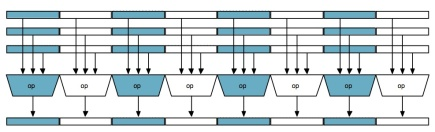
\includegraphics[scale=0.5]{figure/vpu.jpg}
		\end{figure}
	\end{itemize}
\end{frame}


\section{Vectorized}
\subsection{for-loop}
\begin{frame}
    \frametitle{Vecotrized for loop}
    \begin{figure}
		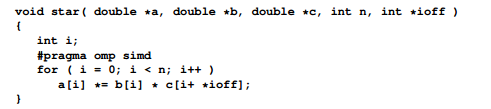
\includegraphics[scale=0.6]{figure/simd1.png}
	\end{figure}
\end{frame}
\subsection{function}
\begin{frame}
    \frametitle{Vecotrized function}
    \begin{figure}
		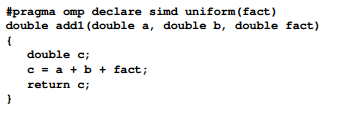
\includegraphics[scale=0.6]{figure/add1.png}
	\end{figure}
\end{frame}
\begin{frame}
    \frametitle{Vecotrized function}
    \begin{figure}
		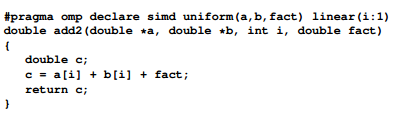
\includegraphics[scale=0.6]{figure/add2.png}
	\end{figure}
\end{frame}



\end{document}
